\Chapter{Specifikáció}

Az előző fejezetben taglaltam milyen fogalmakkal találkozhat a felhasználó a weboldalon. Ebben a fejezetben ismertetem a szoftver tervezésének lépéseit, a felhasznált technológiák technikai hátterét, továbbá bemutatom az általam válaszott grafikus könyvtárat a Chart.JS-t és hogy miért erre esett a döntésem.

\section{Tervezés \cite{agile}}

A programom tervezése során több szempontot vettem figyelemben. Elődleges szempont volt, hogy webalkalmazásként működne legjobban. Ezt az érvet azzal tudom alátámasztani, hogy szem előtt tartva az előnyeit (könnyű hozzáférés, naprakész adatok, jól szemléltethető, skálázható), illetve személyes szakmai tudásomat is a frontend fejlesztés során szereztem. Másodlagos érvemet pedig azzal tudom alátámasztani, hogy az egyetemi tanulmányaim során is webfejlesztésre szakosodtam.

	Az alkalmazás tervezésekor az egyik általam ismert agilis módszertan szerint dolgoztam, amelynek neve \emph{Extreme Programming} (XP). Az Extreme Programming egy specifikus keretrendszer, amelynek célja nem csak a kiváló minőségű szoftver(ek) előállítása, hanem az egész folyamat megkönnyítése is a fejlesztő számára.  A fejlesztési folyamatomatot 5 fázisra lehet bontani. \\

\textbf{Tervezés (planning)}
\begin{itemize}
\item Piackutatás
\item Funkciók meghatározása
\item Szerver-kliens architektúra megtervezése
\item Felhasználandó technológiák
\end{itemize}

\textbf{Elemzések (analysis)}
\begin{itemize}
\item Alkalmazás struktúrákra felosztása
\item Elkészüléshez szükséges idő meghatározása
\item Szakmai tudás felmérése
\item Erőforrás tervezés fejlesztői oldalon
\end{itemize}

\textbf{Design}
\begin{itemize}
\item A feladatok lebontása
\item Összpontosított megjelenés létrehozása és végrehajtása
\end{itemize}

\textbf{Végrehajtás (execution)}
\begin{itemize}
\item Kódolás
\item Kész egységek tesztelése
\item Hibajelentés generálása
\item Iteráció közbeni és végi áttenkintés
\item Folyamatfejlesztések
\end{itemize}

\textbf{Zárás (closure)}
\begin{itemize}
\item Az elkészült termék üzembe helyezése
\item Felhasználói kézikönyv
\item Végső tesztelés
\end{itemize}

\section{Felhasznált technológiák}

\subsection{HTML5}
Mivel a programom online felületre lett tervezve, annak szerkezeti felépítése HTML-ben íródott. A HTML azaz Hypertext Markup Language, magyarul hipertext jelölő nyelv, egy leíró nyelv, amely egy weblap felépítését specifikálja az internetes böngészők felé. Ahogy nevében is láthatjuk, nem egy programozási nyelv, ez azt jelenti, hogy nem programozási logikák megírására, vagy adatok kezelésére használjuk, hanem különböző utasításokkal meghatározzuk az oldalunk struktúráját. \\

\begin{figure}[h]
\centering
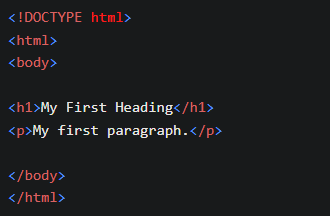
\includegraphics[scale=0.8]{images/htmlExample.png}
\caption{HTML felépítés és elemek megjelenítése}
\end{figure}

\subsubsection{HTML Canvas} 

Canvas elem a HTML5 része és lehetővé teszi két dimenziós alakzatok és dinamikus bittérképek megjelenítését. Több elterjedt 2D API-khoz hasonló rajzfunkciók teljes készletén keresztül érheti el a felhasználni kívánt területet, ezzel elérhetővé téve a dinamikusan generált grafikákat. Főbb felhasználási területe: grafikonok, animációk, játékok és képalkotás.

Mivel grafikonok megvalósításához elengedhetetlen, ezért az én applikációm részét is képezi. A Canvas elem a következőképpen épül fel:
\begin{figure}[h]
\centering
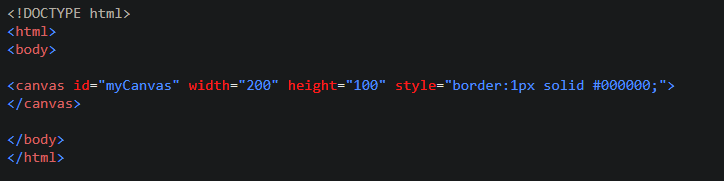
\includegraphics[scale=0.7]{images/canvasExample.png}
\caption{Egy üres négyzet, megvalósítva Canvas elem által}
\end{figure}

\subsection{CSS}

Ahhoz, hogy a HTML által definiált oldalunkon megjelenjenek a kívánt elemek és ezeket jól olvashatóan és igényesen tudjuk megformázni, szükségünk van egy olyan nyelvre, ami a HTML elemekre tud hivatkozni, és különböző nézeti tulajdonságokat tud neki átadni. Ezen célra alkalmas a CSS azaz Cascading Style Sheets, magyarul lépcsőzetes stíluslapok, egy leíró nyelv, amely a HTML elemek megjelenítését, azok stílusát (például: elhelyezkedés, betűszín, karakter formátumok stb.) írj a le a böngésző számára. 

	Különböző választókkal jelölhetünk ki elemeket, azok nevére, osztályára vagy típusára hivatkozva. A lépcsőzetesség arra utal, hogy mely választók vannak priorizálva a weblap megjelenítésének szempontjából. Ez fontos, hisz összetett weblapok esetén többszáz CSS szabály is használatban lehet. \newline
	CSS stílusokat megadhatunk különféle eljárások szerint. \aref{fig:css} \\

	Közvetlenül egy HTML elemen keresztül pontosvesszőkkel elválasztva. Ezt a változatot \emph{sorközi stílus}nak (inline CSS) nevezzük. \\

	Használhatjuk \emph{belső stílus}ként (internal CSS), amely egyedi kinézetet biztosít egyetlen dokumentumhoz. A HTML <head> részében kell meghatározni <style> címkén belül. \\

	Szakmailag legelterjedtebb felhasználása a \emph{külső stílus} (external CSS). A külső stíluslapot általában akkor használjuk, ha több oldalon szeretnénk változtatni. Ideális erre az állapotra, mert megkönnyíti a teljes webhely megjelenésének megváltoztatását egyetlen fájl módosításával. Fejrészen belül elhelyezzük <link> címkék közé a külső fájl forrását, amiben a kódunk szerepel.

\begin{figure}[h]
\centering
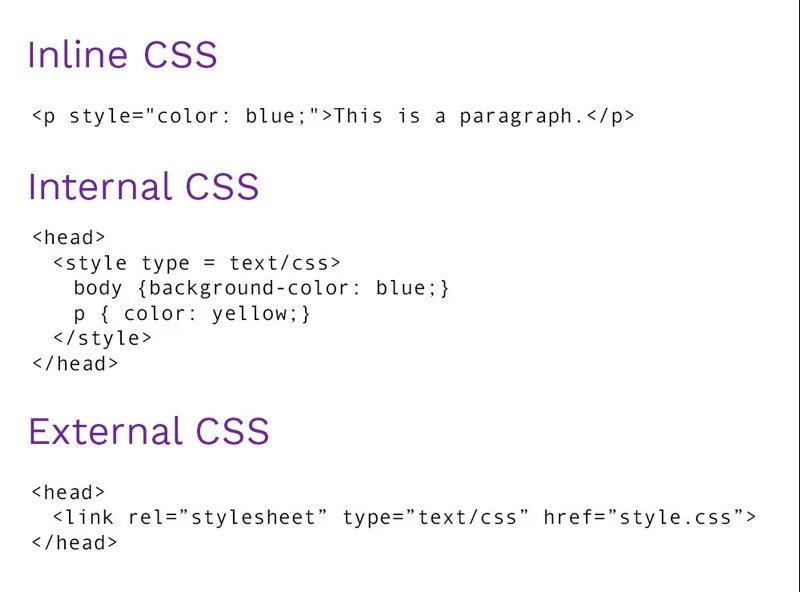
\includegraphics[scale=0.5]{images/cssTypes.png}
\caption{Különböző CSS elérési útvonalak. (forrás: \cite{cssTypes})}
\label{fig:css}
\end{figure}

\subsubsection{Bootstrap5}

A Bootstrap egy ingyenes, nyílt forráskódú frontend fejlesztői keretrendszer webhelyek és webes alkalmazások létrehozásához. Úgy tervezték, hogy lehetővé tegye a webhelyek reszponzív fejlesztését , és a Bootstrap szintaxis gyűjteményt biztosít a sablontervekhez, így a fejlesztőknek csak be kell illeszteni a kódot egy előre meghatározott CSS-keretrendszerbe (grid). Ez a rendszer 12 oszlopos rácsrendszert használ, ezáltal egy reszponzív weboldalt több módon egyenletesen lehet felosztani, ahogy az eszköz nézete megváltozik különféle felbontásban. 

\begin{figure}[h]
\centering
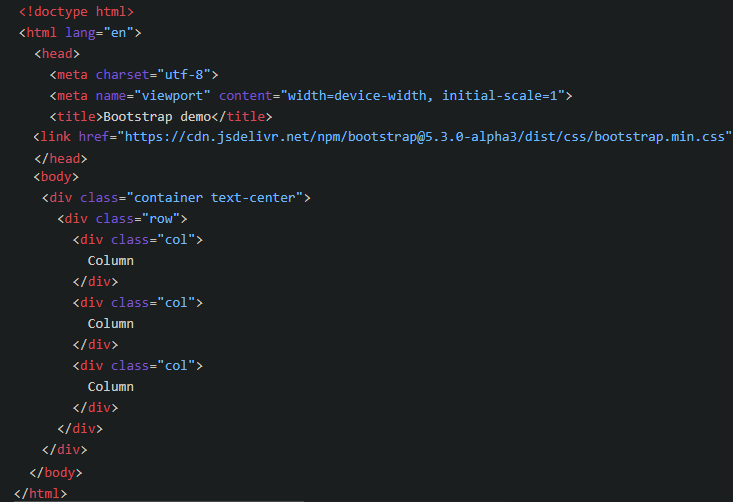
\includegraphics[scale=0.5]{images/bootstrap.png}
\caption{Bootstrap beillesztése HTML dokumentumban és rácsrendszer felosztása }
\end{figure}

\paragraph{Rácsrendszer:}

A rácsrendszerek olyan segédeszközök, amelyeket a tervezők a nehezen átlátható weboldalak megoldásaként valósították meg, hogy az információk rendezettek legyenek és következetes felhasználói élményt biztosítsanak a felhasználók számára. Logikáját tekintve szakított az informatikában gyakran használt decimális számokkal, mivel ezen számokat nem lehet felezni, harmadolni, úgy, hogy egész számokat kapjunk. Így merült fel az a meglátás, miszerint a tároló konténert 12 egyenlő részre osztja fel. Szabadon beállíthatjuk az adott sor(ok), vagy oszlop(ok) milyen szélességgel rendelkezzenek, esetleg a tároló kontéren mekkora részének feleljen meg a képernyőn.

\begin{figure}[h]
\centering
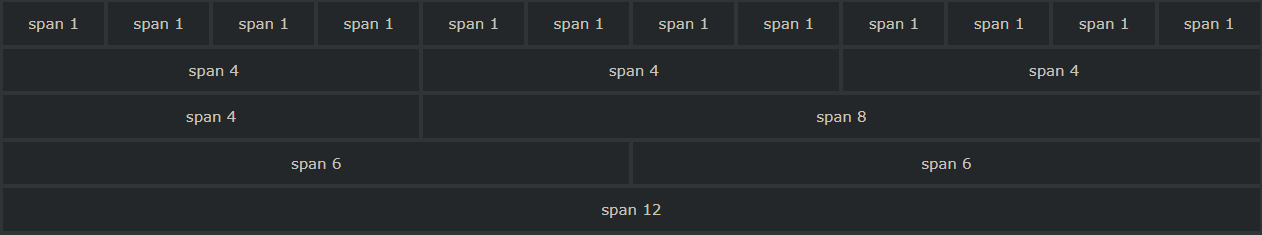
\includegraphics[scale=0.4]{images/gridSystem.png}
\caption{12 oszlopos rácsrendszer felosztása (forrás: \cite{gridSystem})}
\end{figure}

\subsubsection{Font Awsome}

A legegyszerűbb módja annak, hogy figyelemfelkeltő ikonokat helyezzünk el weboldalunkon, ha ikon készletet használunk. Én a Font Awsome internetes ikonkönyvtárát és eszközkészletét használtam fel.

\subsection{NodeJS \cite{nodeJS}}

A Node.js egy nyílt forráskódú, többplatformos futási környezet amiben a gépünkön JavaScript kódot tudunk végrehajtani. Széles körben használják szerveroldali programozáshoz, így a fejlesztők használhatják a JavaScriptet kliensoldali és szerveroldali kódokhoz anélkül, hogy további nyelvet kellene megtanulniuk. Általában egy bizonyos címen és porton figyel az szerver, és mikor kérést kap, elvégzi a leprogramozott funkciókat, majd tétlen állapotban várakozik a következő hívásig. Mivel a Node.js nem folytat közvetlenül kimeneti, vagy bementi műveleteket, így erőforrások blokkolása nem merül fel, ezáltal nem kell félni, hogy a program elakad. Tehát a Node.js ideális interaktív megjelenítő alkalmazások fejlesztésére. \\

\subsubsection{Node Package Manager}

A Node.js futtatásához Node Package Manager (NPM), azaz Node Csomagkezelőt alkalmazunk. Az NPM egy nyílvántartott adatbázis, amelyben szotfverek és a hozzájuk található metaadtok szerepelnek. Három részre lehet felosztani, úgy mint weboldal kezelés, parancssori felület és nyilvántartás.

\subsubsection{Express.JS}

Az Express.js egy Node.js backend keretrendszer, amelyet arra terveztek, hogy az API webalkalmazásait gyorsan és platformokon átívelő almazásokat készítsen, és megkönnyítse a node js-t dolgát. Webes alkalmazások és RESTful API-k építésére tervezték anélkül, hogy bármiben is korlátozná a szerver funkcióit.

\subsection{JavaScript \cite{wikiJS}}

A JavaScript, amelyet gyakran JS-ként is szoktak említeni, egy olyan többparadigmás, dinamikus programozási nyelv, ami lehetővé teszi, hogy a weblapokon komplex funkciókat valósíthassunk meg HTML és CSS használatával. A webhelyek majdnem 100\%-a JavaScriptet használ az elsőrendű függvényeivel, továbbá az alacsony erőforrásigényével. Támogatja a prototípus-alapú objektumorientációval és első osztályú funkciókkal rendelkező kódolást, továbbá az eseményvezérelt, funkcionális és kötelező programozási stílusokat. 

Működését tekintve, nem típusos nyelv, így nem szükséges a változókat deklarálni használat előtt, a megfelelő típust futás közben veszi fel. A JavaScriptet támogató böngésző betölti a HTML oldalt, amennyiben script kód található benne a JavaScript elemző motor kerül előtérbe és a script kód betöltődik. Alkalmazásprogramozási felületekkel (API-kkal) rendelkezik a szöveggel, dátumokkal, reguláris kifejezésekkel való munkához. A legnépszerűbb futásidejű rendszer erre a felhasználásra a Node.js. \\
(Bár a Java és a JavaScript nevüket és szintaxisukat tekintve hasonlóak, a két nyelv különbözik, és nagymértékben eltér egymástól.)


\subsubsection{JQuery}

A jQuery egy nyílt forráskódú, gazdag JavaScript-keretrendszer, amely leegyszerűsíti a HTML/CSS-dokumentumok, pontosabban a Dokumentum Objektum Model (DOM) és a JavaScript közötti interakciókat. Szintaxisát úgy tervezték, hogy megkönnyítse a dokumentumban való navigálást, kezelést, a DOM- elemek kiválasztását, az animációk létrehozását, az események kezelését és az Aszinkron JavaScript XML (Ajax)- alkalmazások fejlesztését.

	 A jQuery lehetőséget biztosít, a fejlesztők számára, hogy absztrakciókat hozzanak létre alacsony szintű interakcióhoz és animációhoz, fejlett effektusokhoz és magas szintű, témára alkalmas widgetekhez. A könyvtár moduláris megközelítése lehetővé teszi hatékony dinamikus weboldalak és webalkalmazások létrehozását. \\

\subsubsection{JSON}

A JavaScript Objektum Jelölés (JSON) egy nyílt szabványos,  nyelvtől független fájlformátum és adatcsere -formátum, amely ember által olvasható szöveget használ az adatobjektumok tárolására és továbbítására. Nagyon elterjedt adatformátum, amelyet sokrétűen alkalmaznak az elektronikus adatcserében, beleértve az adatcserét webes alkalmazások és szerverek között. A JSON két struktúrára épül: \\

Név - érték párok gyűjteménye. Különböző nyelveken ez objektumként , rekordként, struktúraként, szótárként, hash-táblaként, kulcsos listaként vagy asszociatív tömbként valósul meg .
Az értékek listája rendezett. Ezen értékek lehetnek, sztingek, számok,  másik JSON, tömbök, vagy boolean értékek.
A .json fájlnevet ezen objektumok kiterjesztésére használják, nem csak JavaScript programozási nyelven íródott kódokra is. \\

\begin{figure}[h]
\centering
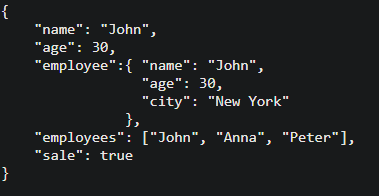
\includegraphics[scale=0.9]{images/jsonExample.png}
\caption{Egy alkalmazott adatai JSON-ként tárolva (forrás: \cite{jsonExample})}
\end{figure}


\section{Miért a Chart.JS? \cite{ChartJS}}

\subsection{ChartJS bemutatása}

A Chart.js egy ingyenes, nyílt forráskódú JavaScript-könyvtár adatvizualizációhoz , amely nyolc diagramtípust támogat : vonal, oszlop, terület, torta ( fánk ), buborék, radar, poláris és szórt diagram. JavaScript nyelven használt beépülő modulokat, diagramtípusokat és testreszabási lehetőségeket kínál. A számtalan beépített modul mellett, a közösség által karbantartott diagramtípusokat is elérhetővé tesz. Ezen felül több diagramtípus kombinálható vegyes diagrammá ugyan azon a Canvas elemen belül.

\begin{figure}[h]
\centering
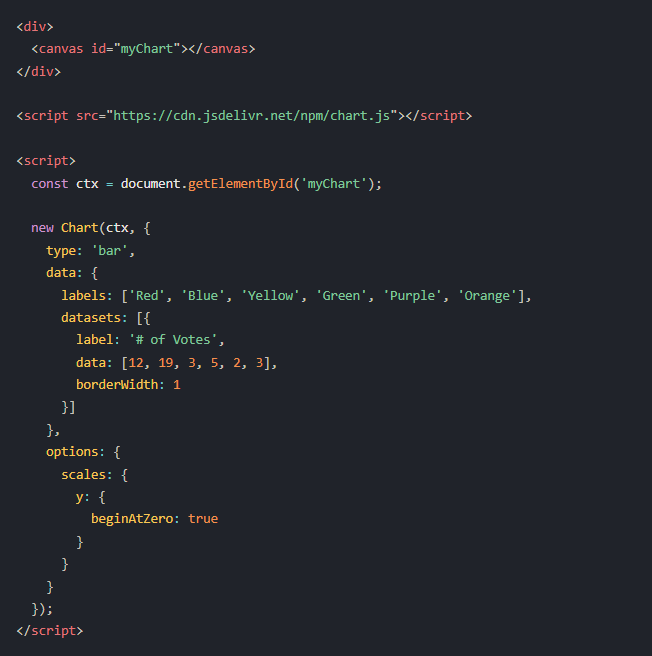
\includegraphics[scale=0.6]{images/chartExample.png}
\caption{diagram létrehozása JSON formátumban (forrás: \cite{ChartJS})}
\end{figure}

\begin{figure}[h]
\centering
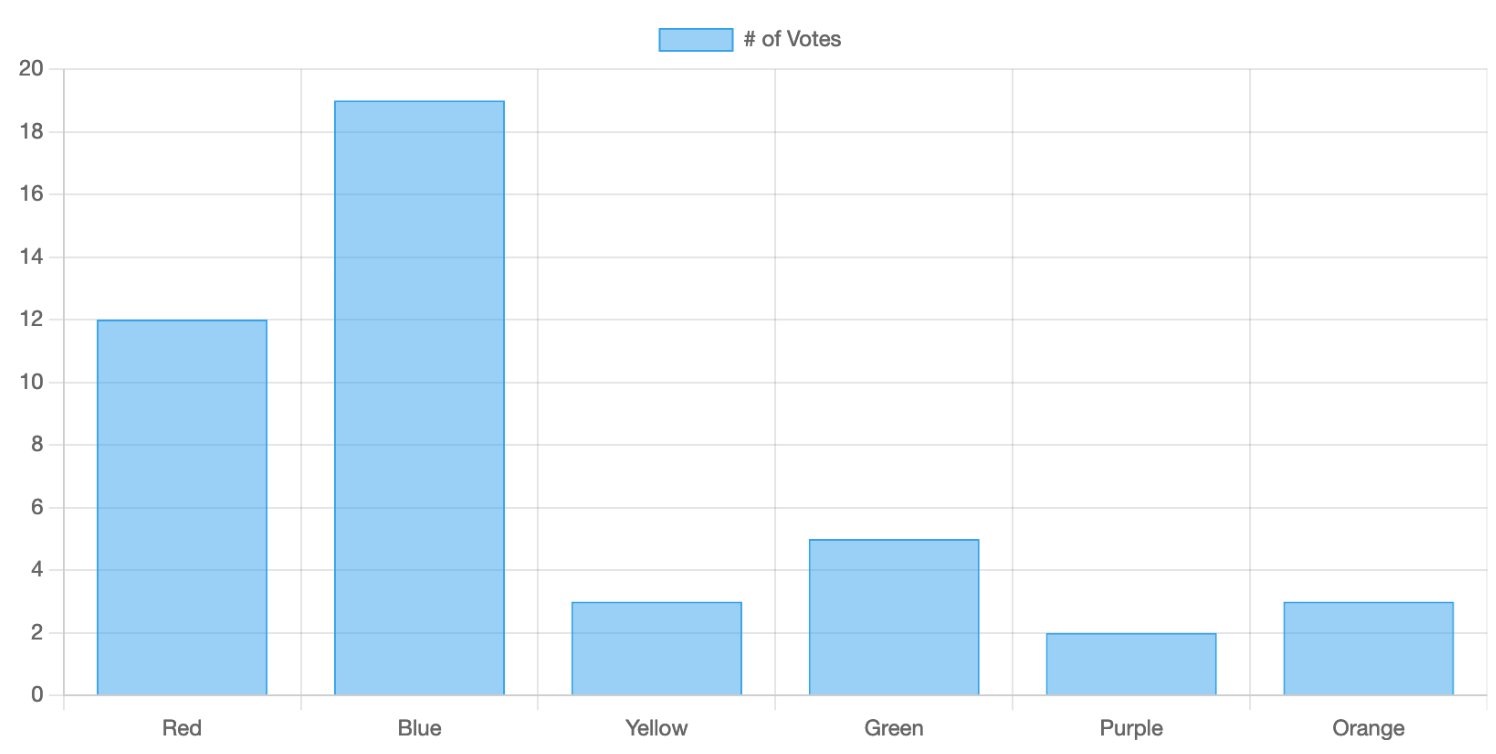
\includegraphics[scale=0.3]{images/barChartJSExample.png}
\caption{Oszlopdiagram ami szavazatok számát mutatja meg (forrás: \cite{ChartJS})}
\end{figure}

\subsection{ChartJS összehasonlítása más grafikus könyvtárakkal \cite{wikiChart}}

\subsubsection{Chart.JS összehasonlítása D3.JS keretrendszerrel}
A csillagok száma alapján a GitHubon a második legnépszerűbb JavaScript diagramkönyvtár a D3.js után, amelyet ugyan lényegesen könnyebben használhatónak tartanak, de kevésbé testreszabható, mint az utóbbi. A Chart.js HTML5 Canvas elemen belül jelenik meg, és széles körben elismert, mint az egyik legjobb adatvizualizációs könyvtár.
A Chart.js nagymértékben testreszabható, hogy néhányat említsek: egyéni beépülő modulokkal, amelyek segítségével megjegyzéseket, nagyítást vagy húzással hozhat létre, hogy néhány dolgot említsünk 

	A Chart.js a diagramelemeket HTML5 Canvas jeleníti meg, ellentétben számos más, többnyire D3.js-alapú diagramkönyvtárral, amelyek Skálázható Vektor Grafika (SVG)-ként jelennek meg. A Canvas megjelenítés nagyon hatékonyvá teszi a Chart.js-t, különösen nagy adatkészletek és összetett vizualizációk esetén, amelyek egyébként több ezer SVG-csomópontot igényelnének a DOM-fában. Ugyanakkor a Canvas renderelés nem engedélyezi a CSS stílust, ezért ehhez beépített opciókat kell használni, vagy különböző diagramtípusokaz kell létrehozni, hogy a kívánt gráfokat jelenjenek meg. 

	A Chart.js nagyon jól használható nagy adathalmazokhoz. Az ilyen adatkészletek hatékonyan feldolgozhatóak belső formátum használatával, így eredményes az adatok elemzéséhez és normalizálásához. Végül a Chart.js által használt Canvas megjelenítés csökkenti a DOM-fájának terhelését, míg az SVG-megjelenítéshez nagyon erőforrás igényes tud lenni. 

\paragraph{ChartJS előnyei}

\begin{itemize}
\item Mivel a Chart.js egy JavaScript könyvtár, így lehetővé teszi, hogy bármilyen választott JS keretrendszerrel használjuk, mint például az Angular.js vagy a React.js..
\item Használata könnyű és minimális fejlesztési ismeretet igényel.
\item Nyílt forráskódú, így csak a meglévő könyvtárat kell felhasználni és nem a fejlesztőnek kell mindent felépíteni.
\item World Wibe Web Consortion (W3C) szabványt követi, így a használatához nincs szükség más böngészőhöz tartozó technológiára, vagy bővítményre.
\item Több megjelenítő eszközzel ellentétben 8 féle diagram megjelenítését engedélyezi.
\item Adatok hatákony manipulálását teszi lehetővé. Rendkívül gyorsan jelenik meg és saját animációkkal rendelkezik.
\item Kiváló dokumentációval van ellátva.
\end{itemize}
